\begin{figure}[!ht]
\begin{center}
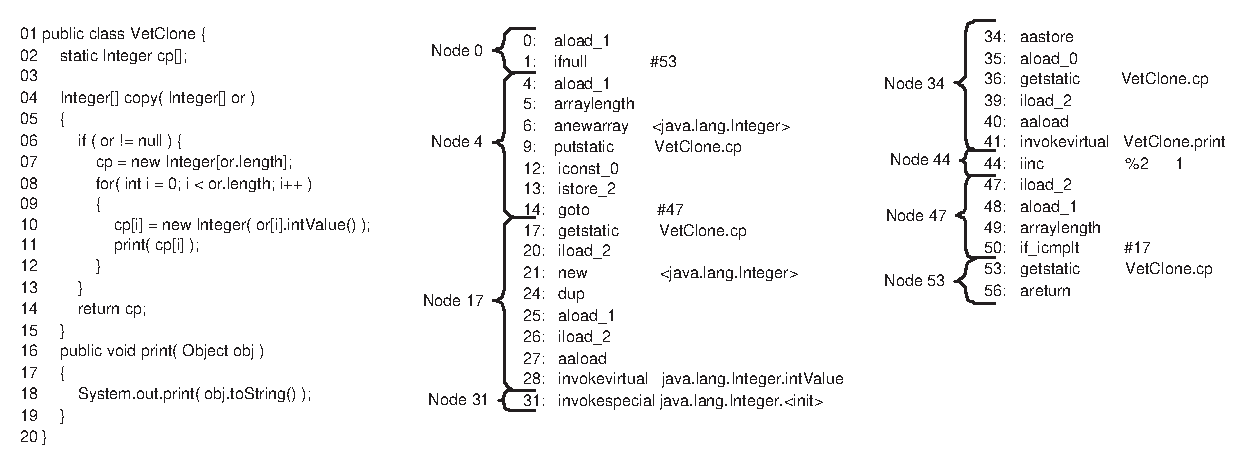
\includegraphics[scale=0.70]{fig/fig-bytecode2.eps}
\caption{Example of variable definition and use for vector and
vector components.}\label{fig-bytecode2}
\end{center}
\end{figure}


\begin{comment}
01 public class VetClone {
02     static Integer cp[];
03
04     Integer[] copy( Integer[] or )
05     {
06         if ( or != null ) {
07             cp = new Integer[or.length];
08             for( int i = 0; i < or.length; i++ )
09             {
10                 cp[i] = new Integer( or[i].intValue() );
11                 print( cp[i] );
12             }
13         }
14         return cp;
15     }
16     public void print( Object obj )
17     {
18         System.out.print( obj.toString() );
19     }
20 }

0:    aload_1
1:    ifnull        #53
4:    aload_1
5:    arraylength
6:    anewarray     <java.lang.Integer>
9:    putstatic     VetClone.cp
12:   iconst_0
13:   istore_2
14:   goto          #47
17:   getstatic     VetClone.cp
20:   iload_2
21:   new           <java.lang.Integer>
24:   dup
25:   aload_1
26:   iload_2
27:   aaload
28:   invokevirtual java.lang.Integer.intValue
31:   invokespecial java.lang.Integer.<init>
34:   aastore
35:   aload_0
36:   getstatic     VetClone.cp
39:   iload_2
40:   aaload
41:   invokevirtual VetClone.print
44:   iinc          %2      1
47:   iload_2
48:   aload_1
49:   arraylength
50:   if_icmplt     #17
53:   getstatic     VetClone.cp
56:   areturn
\end{comment}
